\documentclass[RNAAS]{aastex62}

\newcommand{\vdag}{(v)^\dagger}
\newcommand\aastex{AAS\TeX}
\newcommand\latex{La\TeX}

\submitjournal{RNAAS}

\shorttitle{Non-Detection of Helium for WASP-12b}
\shortauthors{Kreidberg \& Oklop\v{c}i\'{c}}

\begin{document}

\title{Non-Detection of a Helium Exosphere for the Hot Jupiter WASP-12b}


\author{Laura Kreidberg}
\affiliation{Harvard-Smithsonian Center for Astrophysics, 60 Garden Street, Cambridge, MA 02138}
\affiliation{Harvard Society of Fellows, 78 Mount Auburn Street, Cambridge, MA 02138}

\author{Antonija Oklop\v{c}i\'{c}}
\affiliation{Harvard-Smithsonian Center for Astrophysics, 60 Garden Street, Cambridge, MA 02138}
A helium exosphere was recently detected around the exoplanet WASP-107b, a
low-density, warm Neptune \citep{spake18}, based on absorption features from metastable helium at $10833\,\mathrm{\AA}$ \citep[predicted
by][]{seager00,oklopcic18}. The helium feature provides a new probe of atmospheric escape that is
advantageous in several ways: (1) it is observable with near-infrared facilities
(in contrast to other signposts of atmospheric escape that appear in the
ultraviolet) and (2) it is minimally affected by interstellar absorption,
thereby opening the door to studying atmospheric escape in a greater number of systems.

Inspired by the WASP-107b detection, we searched archival HST observations of
another evaporating exoplanet, WASP-12b, for signs of a helium exosphere.
WASP-12b is a promising 
candidate for this search because it is one of the hottest known hot
Jupiters \citep[$T_\mathrm{eq} = 2500$ K;][]{hebb09}. At this level of intense irradiation, theory predicts a high rate of escaping atoms and molecules from the planet's atmosphere, and indeed, transit observations in the ultraviolet have revealed a patchy cloud of escaping material \citep{nichols15}.  

For this Note, we reanalyzed three transits of WASP-12b observed with the
Hubble Space Telescope/Wide Field Camera 3 G102 grism \citep[originally published in][]{kreidberg15b}.  In our analysis, we used the same methodology as
\cite{kreidberg15b}, except with different spectral binning to include a narrow
band ($70\,\mathrm{\AA}$, the spectrograph's native resolution) centered on the
He feature, with two wider bands at adjacent wavelengths. 
The transmission spectrum (shown in Figure\,\ref{fig:spectrum}) is consistent with that reported in
\cite{kreidberg15b} and shows no evidence for variability between epochs.  Surprisingly, there
is no significant increase in transit depth at $10833\,\mathrm{\AA}$.  

To estimate the expected absorption signal of WASP-12b at $10833\,\mathrm{\AA}$,
we used the theoretical model described in \cite{oklopcic18}.
In this 1D model, we assumed the thermosphere of the planet is composed of atomic hydrogen and helium in 9:1 number
ratio. For the thermospheric density and velocity profiles we adopted the
isothermal Parker wind model, assuming the gas temperature of $T=10^4$~K and the
total atmospheric mass loss rate of $4\times 10^{11}$~g~s$^{-1}$ \citep[based on
the results of hydrodynamic simulations of atmospheric escape in WASP-12b
by][]{salz16}. We used the solar irradiance spectrum as the input spectrum. We
considered two cases: one that includes all the evaporating gas predicted from
the Parker wind model (Model A), and the other
that only includes gas within the planet's Roche radius (Model B), to account
for the possibility of dissipation of gas as it escapes the planet's gravitational influence.

Model A predicts an equivalent width for the helium feature of
$0.056\,\mathrm{\AA}$, which is ruled out by the observed spectrum at
$5.2\sigma$ confidence (see Figure\,\ref{fig:spectrum}). By contrast, Model B
predicts a smaller equivalent width ($0.003\mathrm{\AA}$) that is consistent with the data, suggesting rapid dissipation of the gas cloud.  In addition, another possible explanation for the absence of a large helium feature is that WASP-12 may be faint in the EUV. The star has an unusually low activity level, which has been attributed to a shroud of material accreted from the evaporating planet \citep{haswell17}. If the EUV flux is lower than that of the Sun, the population of helium in the metastable state will be relatively depleted, shrinking the amplitude of the $10833\mathrm{\AA}$ feature.

%It is possible that the geometry of the gas flow is different for WASP-12b than WASP-107b,
%thanks to the planet's faster orbital velocity and higher irradiation.


In conclusion, we find that WASP-12b has no evidence for a helium exosphere, but the
significance of the result is dependent on the assumed geometry of the
evaporating gas cloud as well as the input stellar spectrum.  Both of these factors should be considered in the design of future searches for helium exospheres.

\begin{figure*}[b!]
\begin{centering}
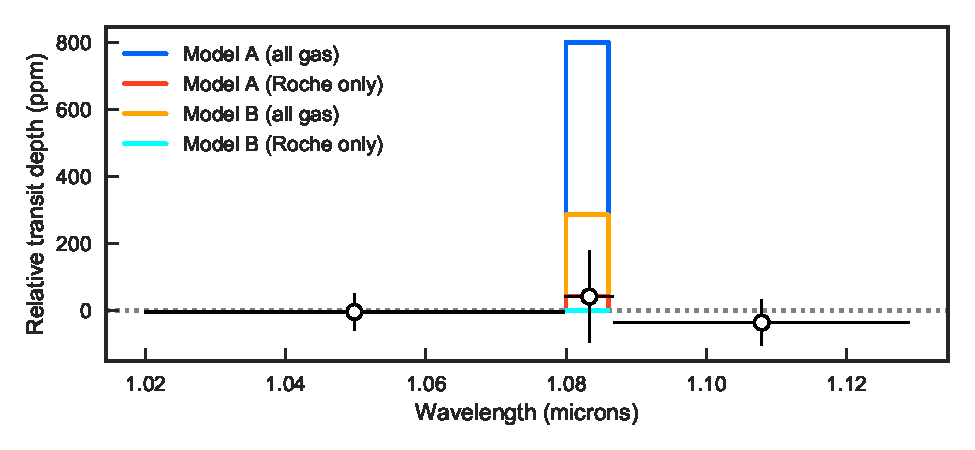
\includegraphics[width = 0.75\textwidth]{Figures/fig1.pdf}
\caption{Transmission spectrum of WASP-12b, compared to model predictions for
the strength of the $10833\mathrm{\AA}$ helium feature.}
\end{centering}
\label{fig:spectrum}
\end{figure*}


\bibliographystyle{aasjournal}
\bibliography{ms.bib}

\end{document}

% End of file `sample62.tex'.
